 \chapter[Metodologia]{Metodologia}

 \section{Desenvolvimento geral}
Visando realizar a otimização estrutural de um painel reforçado utilizando os parâmetros de laminação, realizou-se uma sequência de passos conforme segue:
\begin{enumerate}
  \item Análise teórica de um painel reforçado de material metálico utilizando a metodologia do \emph{Fator de Eficiência de Farrar} proposta por \cite{niu1997airframe}
  \item Otimização de um painel reforçado de material metálico utilizando o \emph{MSC Nastran} e comparação dos resultados obtidos com o resultado teórico obtido no item anterior. Nesta etapa visou-se obter a validação o método de otimização utilizado para assim poder aplicá-lo em outros paineis reforçados;
  \item Otimização de um painel reforçado de material composto utilizando o \emph{MSC Nastran} e comparação dos resultados obtidos com os resultados obtidos para um painel reforçado de material metálico.
\end {enumerate}

As seções seguintes descrevem a metodologia utilizada com mais detalhes e apresentam os modelos das otimizações realizadas e o capítulo seguinte contém os resultados obtidos.

\section{Análise teórica de um painel reforçado}
Visando realizar a análise teórica de um painel reforçado fabricado em material metálico, assume-se algumas proposições como segue e considera-se um painel conforme mostrado na \autoref{fig_StiffenedPanels}.

\begin{itemize}
\item Painel suficientemente largo para permitir que seja tratado como uma simples coluna, ou seja, não há restrições impostas nas bordas longitudinais do painel;
\item O painel possui uma fixação de apoio no final da sua estrutura, em relação ao comprimento L. Deve-se levar em consideração este comprimento como sendo o o comprimento efetivo do painel, e não o comprimento da báia;
\item As nervuras não colocam restrições à flambagem.
\end{itemize}

\begin{figure}[h]
	\caption{\label{fig_StiffenedPanels}Típico painel reforçado.}
  \centering
  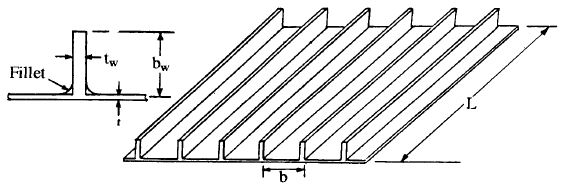
\includegraphics[scale=1.0]{figura/StiffenedPanel}
	\legend{Fonte: \cite{niu1997airframe}}
\end{figure}
\

Nota-se que\

$t$ -  Espessura do revestimento \

$b$ - Largura entre reforçadores \

$t_w$ - Espessura do reforçador \

$b_w$ - Altura do reforçador \

$L$ - Comprimento efetivo \
\

A \autoref{fig_InitialBuckling} mostra a tensão de flambagem inicial de diversas combinações de paineis reforçados, como razão entre $\dfrac{f_i}{f_o}$, considerando a seguinte notação.

\begin{figure}[h]
	\caption{\label{fig_InitialBuckling}Tensão inicial de flambagem.}
  \centering
  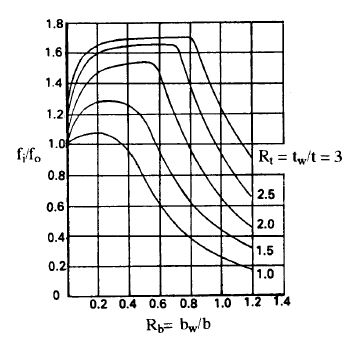
\includegraphics[scale=1.0]{figura/InitialBuckling}
	\legend{Fonte: \cite{niu1997airframe}}
\end{figure}
\
$f$ - Tensão aplicada\

$f_E$ - Tensão de instabilidade de Euler\

$f_i$ - Tensão inicial de flambagem do painel\

$f_o$ - Tensão inicial de flambagem de um painel reforçado longo, com espaçamento entre reforçadores (b) e espessura do revestimento (t), simplesmente apoiado ao longo da borda = 3.62$E_t$$(\dfrac{t}{b})^2$\

Segundo \cite{niu1997airframe}, para um dado material, no qual a relação entre $f$ e $E_t$ é conhecida, o \emph{Fator de Eficiência de Farrar} pode ser dado por:

\begin{equation} \label{Farrar}
F = f(\dfrac{L}{N E_t})^{0.5}
\end{equation}
Onde

$N$ - Carga por unidade de comprimento do painel (lbs/in)\

$E_t$ - Módulo tangente (psi)

\begin{figure}[h]
	\caption{\label{fig_plotFarrar}Tensão no painel \emph{vs.} índice estrutural $\dfrac{N}{L}$ para material Al 2024-T3.}
  \centering
  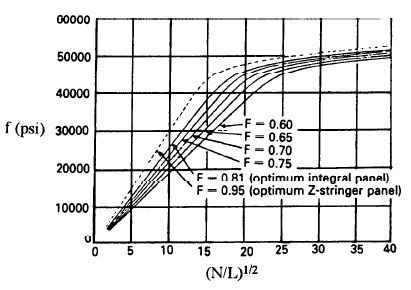
\includegraphics[scale=1.0]{figura/PlotFarrar}
	\legend{Fonte: \cite{niu1997airframe}}
\end{figure}
\

Este fator pode ser utilizado, conforme \autoref{fig_plotFarrar} que mostra para um painel reforçado de Al 2024-T3.

Sabe-se que a tensão incial de flambagem ($f_i$) é dada por:

\begin{equation} \label{InitialBuck}
f_i = (\dfrac{f_i}{f_o})[{3.62E_t(\dfrac{t}{b})^2}]
\end{equation}

E que a tensão de instabilidade de Euler ($f_E$) é dada por:

\begin{equation} \label{InitialEuler}
f_E = {\pi^2}E_t(\dfrac{\rho}{L})^2
\end{equation}

Onde $\rho$ corresponde ao raio de giração do painel reforçado em relação ao seu eixo neutro e tem que:

\begin{equation} \label{giracao}
{\rho^2} = {\dfrac{b^2{R_b}^3R_t}{12(1+R_bR_t)}}(4+R_bR_t)^2
\end{equation}

Em que
\begin{equation} \label{Rb}
R_b = \dfrac{b_w}{b}
\end{equation}
\

\begin{equation} \label{Rt}
R_t = \dfrac{t_w}{t}
\end{equation}

Relacionando a tensão no painel com a intensidade de carga tem-se:

\begin{equation} \label{StressPanel}
f = \dfrac{N}{t(1+R_bR_t)}
\end{equation}

Portanto, impõe-se a condição de que tensão aplicada é igual à tensão inicial de flambagem do painel que é igual à tensão de instabilidade de Euler ($f=f_i=f_E$).

Tomando-se a \autoref{InitialBuck} x \autoref{InitialEuler} x {\autoref{StressPanel}$^2$, obtem-se:

\begin{equation} \label{StressPanel2}
f^4 = \pi^2{E_t}^2(\frac{3.62{\rho}^2f_i}{f_ob^2L^2})[\dfrac{N^2}{(1+R_bR_t)^2}]
\end{equation}

Tirando a raiz quarta de ambos os lados, tem-se:

\begin{equation} \label{StressPanel3}
f = F(\dfrac{NE_t}{L})^{0.5}
\end{equation}

Onde o \emph{Fator de Eficiência de Farrar} vale:

\begin{equation} \label{Farrar_Efficiency}
F = 1.314{\dfrac{{R_b}^3R_t(4+R_bR_t)^{0.25}}{(1+R_bR_t)}}({\frac{f_i}{f_o}})^{0.25}
\end{equation}

\subsection{Limitação de projeto - Espaçamento entre reforçadores}
Considerando um espaçamento entre reforçadores (b) já previamente determinado, devido ao modelo em elementos finitos que foi desenvolvido para as etapas de otimização, tem-se, portanto, uma limitação de projeto. Segundo \cite{niu1997airframe}, para manter o valor de largura entre reforçadores constante (b) ou o valor de espessura do reforçador também constante ($t_w$), tem-se as seguintes relações, que também são plotadas na \autoref{fig_plotstiffener}.

\begin{equation} \label{Farrar_Efficiency_J1}
J_1 = b({\dfrac{E_t}{NL^3}})^{0.25}
\end{equation}

\begin{equation} \label{Farrar_Efficiency_J2}
J_2 = t_w({\dfrac{E_t}{NL^3}})^{0.5}
\end{equation}

No caso deste estudo, considerou-se que a largura entre os reforçadores será constante, visando obter os outros parâmetros geométricos do painel reforçado ótimo.

\begin{figure}[ht]
	\caption{\label{fig_plotstiffener}Curvas para projetos com limitações - Espessura do reforçador ($t_w$) e largura do reforçador (b).}
  \centering
  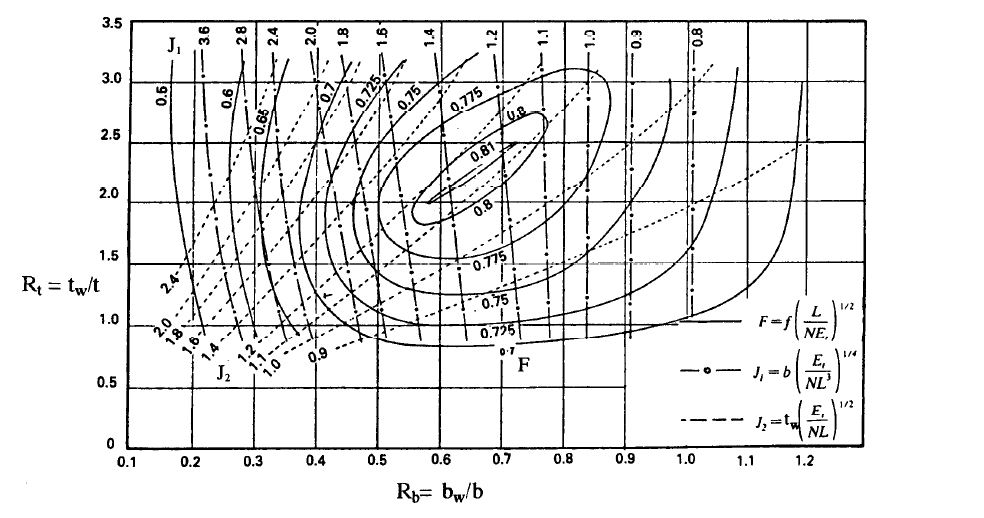
\includegraphics[scale=1.0]{figura/PlotStiffener}
	\legend{Fonte: \cite{niu1997airframe}}
\end{figure}
\

Visando, portanto, projetar um painel reforçado otimizado, seguindo a metodologia de \emph{Fator de Eficiência de Farrar} proposta por \cite{niu1997airframe}, submetido a uma carga de intensidade N (lbs/in), alguns passos foram seguidos:

\begin{itemize}
\item Utilização de valores otimizados \
F=0.81; $R_t$=2.25; $R_b$=0.65z;\
\item Da \autoref{fig_plotFarrar}, encontrou-se o valor de "f" correspondente a carga por largura (N/L), utilizando F=0.81 para o Al 2024-T3 extrudado;
\item Encontrou-se o módulo tangente $E_t$ correspondente ao valor de "f", da curva de módulo tangente do material, conforme \autoref{fig_tangentmodulus};
\item Determinou-se os valores de t, b, $t_w$ e $b_w$, conforme \autoref{Farrar_Efficiency_t} e \autoref{Farrar_Efficiency_tw}.
\begin{equation} \label{Farrar_Efficiency_t}
t = 0.501({\dfrac{NL}{E_t}})^{0.5}
\end{equation}
\begin{equation} \label{Farrar_Efficiency_tw}
t_w = 2.25t
\end{equation}

\end{itemize}

\begin{figure}[ht]
	\caption{\label{fig_tangentmodulus}Curva do módulo de elasticidade tangente para Al 2014-T3 extrudado.}
  \centering
  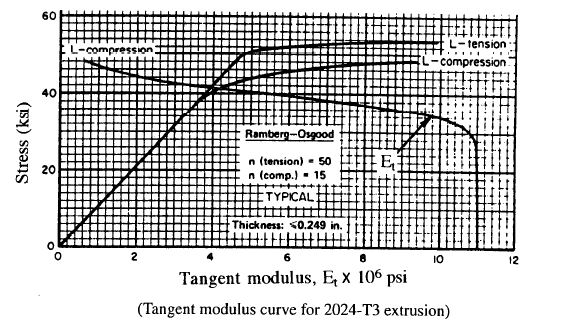
\includegraphics[scale=1.0]{figura/TangentModulus}
	\legend{Fonte: \cite{niu1997airframe}}
\end{figure}

\section{Otimização de um painel reforçado em material metálico}
Realizou-se uma otimização de um painel reforçado em material metálico utilizando o \emph{MSC Nastran}, para que após a validação do otimizador ele pudesse ser aplicado para outros tipos de paineis reforçados, como os painéis em material composto.

\subsection{Modelo em elementos finitos}
Desenvolveu-se um modelo em elementos finitos de um painel reforçado, conforme \autoref{fig_StiffMetal} para realizar a análise de otimização. Este modelo foi desenvolvido utilizando somente um tipo de material, tanto para o revestimento quanto para o reforçador (Al 2024 T3), com as características conforme mostrado na \autoref{tbl:prop_metalico}.

\begin{table}[h]
\centering
\begin{tabular}{ccc}
\toprule
& Propriedades Al 2024-T3 extrudado \\ \midrule
Módulo de elasticidade (E) & $73.7$x$10^3N/mm^2$ & $10.7$x$10^3$ ksi \\
Coeficiente de Poisson ($\nu$) & 0.33 & 0.33\\
Densidade mássica ($\rho$)  & $2.8$x$10^{-3} g/mm^3$ & 0.1 $lb/in^3$ \\
\bottomrule
\end{tabular}
\caption{Propriedades do material metálico. Fonte:\cite{rice2003metallic}}
\label{tbl:prop_metalico}
\end{table}

\begin{figure}[ht]
	\caption{\label{fig_StiffMetal}Modelo do reforçador em material metálico.}
  \centering
  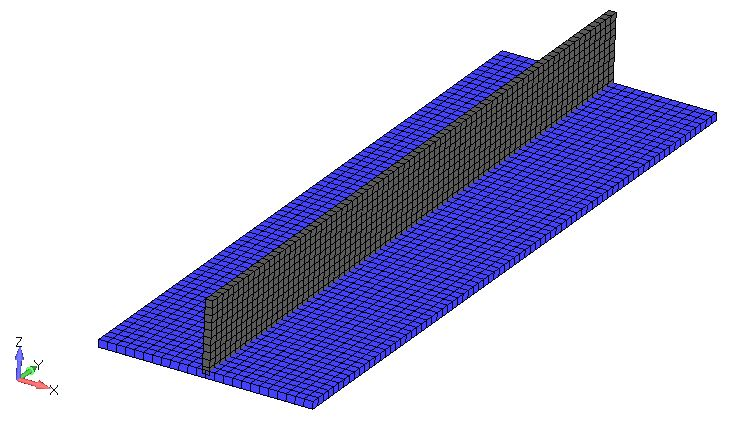
\includegraphics[scale=0.7]{figura/StiffMetal}
	\legend{Fonte: Femap}
\end{figure}
\

O modelo foi desenvolvido com elementos do tipo placa (\emph{PLATE}) para o reforçador e para o revestimento, e com duas propriedades distintas, sendo uma propriedade para o revestimento e outra propriedade para o reforçador, visto que possuem espessuras diferentes.

O painel reforçado foi modelado utilizando somente a idealização de um reforçador e para isso as seguintes condições de contorno foram aplicadas, conforme mostrado na (adicionar figura)%\autoref{fig_StiffMetalConst}.

%begin{figure}[ht]
%	\caption{\label{fig_StiffMetal}Condições de contorno aplicadas no painel reforçado.}
%  \centering
%  \includegraphics[scale=0.7]{figura/CondContorno}
%	\legend{Fonte: Femap}
%\end{figure}
%\

Em relação ao carregamento do aplicado no modelo, definiu-se que o painel reforçado estaria submetido somente a uma carga de compressão, sem cisalhamento. E portanto, aplicou-se essa carga de compressão conforme mostrado na \autoref{fig_StiffMetalLoad},
utilizando um elemento rígido do tipo RBE2 para distribuir a carga igualmente nos nós dos elementos de placa que situam-se em uma extremidade do reforçador.

\begin{figure}[h]
	\caption{\label{fig_StiffMetalLoad}Carregamento aplicado no reforçador em material metálico.}
  \centering
  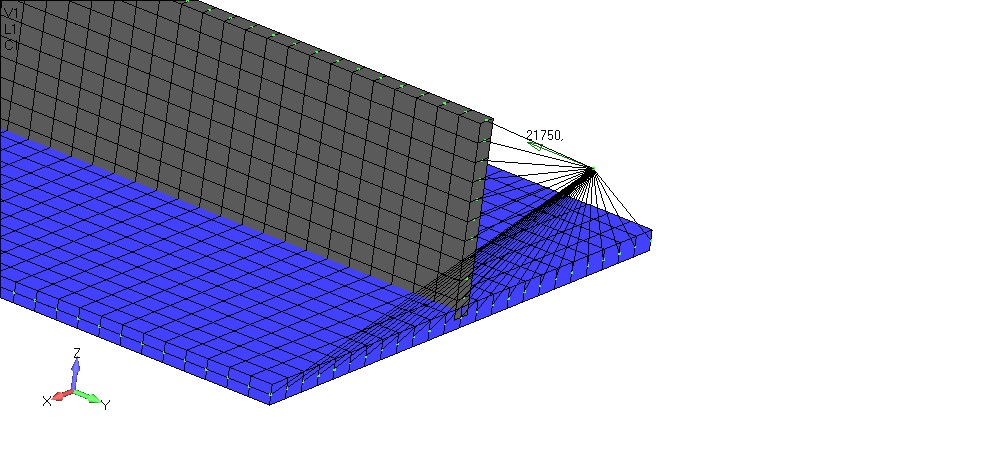
\includegraphics[scale=0.7]{figura/StiffMetalLoad}
	\legend{Fonte: Femap}
\end{figure}
\

\subsection{Otimização}
Em relaçao a otimização, buscou-se como objetivo minimizar o peso da estrutura. Portanto, durante a solução de otimização, mateve-se a carga de compressão constante e variou-se as espessuras do revestimento e do reforçador. Buscou-se, então, uma estrutura que suportasse a carga de compressão, utilizando uma análise de flambagem dentro do otimizador (SOL 105), e que possuíse o menor peso estrutural.

Resumidamente, a otimização possuiu as seguintes características:
\begin{itemize}
\item Função objetivo: minimizar o peso da estrutura;
\item Variáveis de projeto: espessura do revestimento e espessura do reforçador;
\item Respostas de projeto: Cinco (5) primeiros autovalores da solução de flambagem;
\item Restrições de projeto: Autovalores maiores que um (1), ou seja, maiores que a carga aplicada;
\item Soluções utilizadas: Otimização (SOL 200) e Análise de flambagem (SOL 105).
\end{itemize}

\section{Otimização de um painel reforçado em material composto}
Após a realização da otimização do painel reforçado em material metálico, realizou-se a otimização de um painel reforçado em material composto utilizando o \emph{MSC Nastran}.

\subsection{Modelo em elementos finitos}
Similarmente ao modelo para o painel reforçado em material metálico, desenvolveu-se um modelo em elementos finitos de um painel reforçado em material composto, conforme \autoref{fig_StiffComposite} para realizar a análise de otimização.

\begin{figure}[ht]
 \caption{\label{fig_StiffComposite}Modelo do reforçador em material composto.}
 \centering
 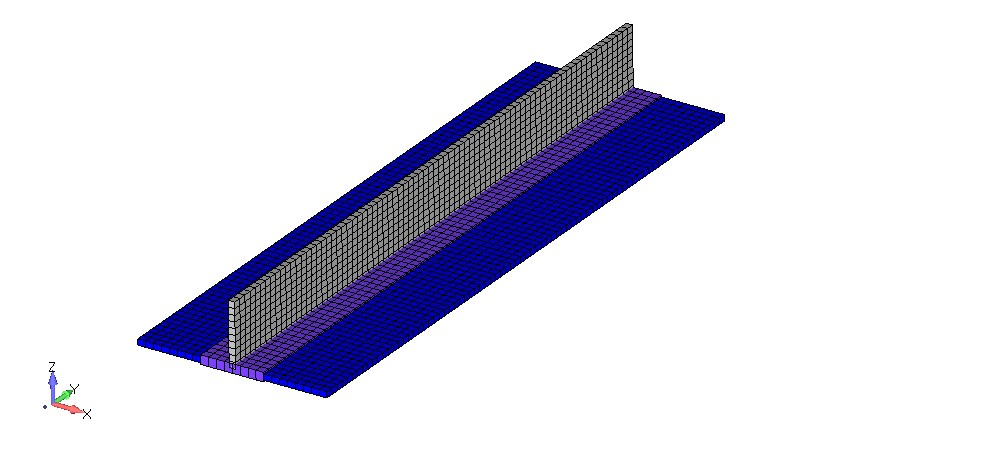
\includegraphics[scale=0.7]{figura/StiffComposite}
 \legend{Fonte: Femap}
\end{figure}
\

Este modelo foi desenvolvido utilizando como material composto o carbono, mas com duas propriedades de materiais distintas. Sendo que tem-se um material exclusivamente para o revestimento e outro para a alma do reforçador. Já a base do reforçador é composta tanto pelo material do revestimento, quanto pelo material da alma do reforçador, conforme ilustrado na \autoref{fig_StiffCompositeMaterial}.

\begin{figure}[ht]
 \caption{\label{fig_StiffCompositeMaterial}Visualização do reforçador em material composto.}
 \centering
 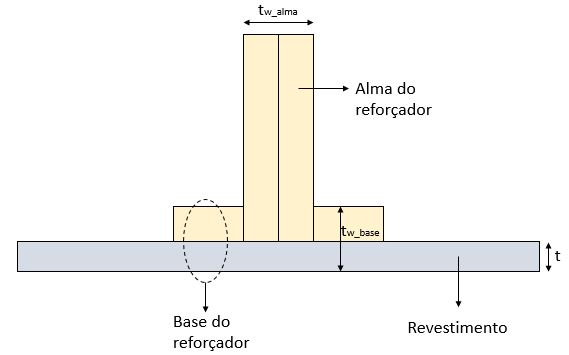
\includegraphics[scale=0.7]{figura/StiffCompositeMaterial}
\end{figure}
\

O modelo foi desenvolvido com elementos do tipo placa (\emph{PLATE}) para o reforçador e para o revestimento, e com duas propriedades distintas, sendo uma propriedade para o revestimento e outra propriedade para o reforçador. Portanto, tem-se uma dada espessura para o reforçador ($t_{w alma}$), uma espessura para o revestimento (t) e uma espessura para a base do reforçador ($t_{w base}$) que é uma relação entre a espessura da alma do reforçador e a espessura do revestimento.

Optou-se por modelar a base do refoçador de material composto visando fazer a conexão entre as propriedades dos materiais da alma do reforçador e do revestimento.

O painel reforçado foi modelado utilizando somente a idealização de um reforçador, as condições de contorno aplicadas no modelo de elementos finitos de reforçador em material composto são as mesmas que foram aplicadas no modelo do reforçador em material metálico, conforme mostrado na (adicionar figura). %\autoref{fig_StiffMetalConst}.

Em relação ao carregamento do aplicado no modelo, definiu-se que o painel reforçado estaria submetido somente a uma carga de compressão, sem cisalhamento. E portanto, aplicou-se essa carga de compressão igualmente àquela aplicada no modelo do reforçador de material metálico, conforme mostrado na \autoref{fig_StiffMetalLoad}. Utilizou-se um elemento rígido do tipo RBE2 para distribuir a carga igualmente nos nós dos elementos de placa que situam-se em uma extremidade do reforçador.

\subsection{Otimização}
Em relaçao a otimização, buscou-se como objetivo minimizar o peso da estrutura. Portanto, durante a solução de otimização, mateve-se a carga de compressão constante e variou-se as espessuras do revestimento e do reforçador. Na otimização do painel reforçado, variou-se também os parâmetros de laminação tanto do revestimento, quanto do reforçador. Buscou-se, então, uma estrutura que suportasse a carga de compressão, utilizando uma análise de flambagem dentro do otimizador (SOL 105), e que possuíse o menor peso estrutural.

Resumidamente, a otimização possuiu as seguintes características:
\begin{itemize}
\item Função objetivo: minimizar o peso da estrutura;
\item Variáveis de projeto: espessura do revestimento, espessura do reforçador e os parâmetros de laminação do revestimento e do reforçador;
\item Respostas de projeto: Cinco (5) primeiros autovalores da solução de flambagem;
\item Restrições de projeto: Autovalores maiores que um (1), ou seja, maiores que a carga aplicada;
\item Soluções utilizadas: Otimização (SOL 200) e Análise de flambagem (SOL 105).
\end{itemize}
